\documentclass{article}
\usepackage{amsmath}
\usepackage{tikz}
\usepackage{pgfplots}
\pgfplotsset{compat=1.18}

\begin{document}
An ordinary mathematical formula: $\int_0^1 x^2\,dx=\frac{1}{3}$.

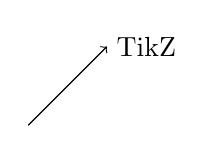
\begin{tikzpicture}
  \draw[->] (0,0) -- (1,1) node[right] {TikZ};
\end{tikzpicture}

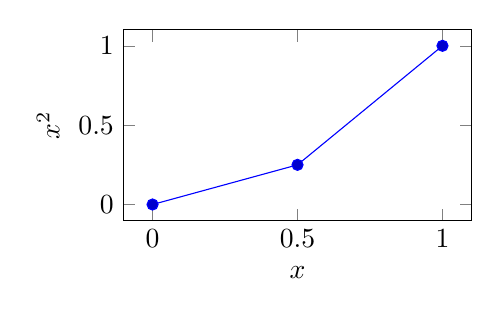
\begin{tikzpicture}
  \begin{axis}[width=6cm, height=4cm, xlabel={$x$}, ylabel={$x^2$}]
    \addplot coordinates {(0,0) (0.5,0.25) (1,1)};
  \end{axis}
\end{tikzpicture}
\end{document}
